%%%%%%%%%%%%%%%%%% DOCUMENT SETUP %%%%%%%%%%%%%%%%%%


% Required IEEE parameters
\documentclass[letterpaper, 10pt, conference]{ieeeconf} % set document type
\IEEEoverridecommandlockouts                              % for \thanks command
\overrideIEEEmargins                                      % use for \addtolength to normalize column lengths


% Packages
\usepackage{graphicx} % allows additional graphics formats
  \graphicspath{ {./images/} }
\usepackage{amsmath}   % assumes amsmath package installed
  \allowdisplaybreaks[1] % allow eqnarrays to break across pages
\usepackage{amssymb}   % assumes amsmath package installed 
\usepackage{url}       % format hyperlinks correctly
\usepackage{rotating}  % allow portrait figures and tables
\usepackage{subfigure} % allow matrices of figures
\usepackage{float}     % allows H option on floats to force here placement
\usepackage{multirow}  % allows merging of rows in tables
\usepackage{tabularx}  % allows fixed width tables
\usepackage{ctable}    % modifies \hline for use in table
\usepackage{bm}        % allow bold fonts in equations
\usepackage{wrapfig}   % allow text wrapping round figures

\usepackage{stfloats}  % control placement of floats
%\usepackage[utf8]{inputenc}
%usepackage[english]{babel}
\usepackage[backend=biber,style=ieee,maxbibnames=3,bibencoding=utf8]{biblatex}   
\addbibresource{references.bib}
% allow bibliography control 
%\usepackage[backend=biber,style=ieee,maxbibnames=3,bibencoding=utf8]{biblatex}   % allow bibliography control 
 % \addbibresource{journal_abbreviations.bib}
%  \addbibresource{references.bib}  
\usepackage{siunitx}
\usepackage{placeins}

% Custom commands
\newcommand{\matlab}{\emph{\sc{Matlab}}}
\newcommand{\maple}{\emph{\sc{Maple}}}
\newcommand{\simulink}{\emph{\sc{Simulink}}}
\newcommand{\dc}{d.c.}
\newcommand{\ac}{a.c.}
\newcommand{\rms}{RMS}
\newcommand{\wgn}{{\tt wgn}}
\newcommand{\sus}[1]{$^{\mbox{\scriptsize #1}}$}
\newcommand{\sub}[1]{$_{\mbox{\scriptsize #1}}$}
\newcommand{\chap}[1]{Chapter~\ref{#1}}
\newcommand{\sect}[1]{Section~\ref{#1}}
\newcommand{\fig}[1]{Fig.~\ref{#1}}
\newcommand{\tab}[1]{Table~\ref{#1}}
\newcommand{\equ}[1]{(\ref{#1})}
\newcommand{\appx}[1]{Appendix~\ref{#1}}
\newcommand{\degree}{\ensuremath{^\circ}}
\newcommand{\Vrms}{V\sub{\rms}}
\newcommand{\Vpp}{V\sub{pp}}
\newcommand{\otoprule}{\midrule[\heavyrulewidth]}         
\newcolumntype{Z}{>{\centering\arraybackslash}X}  % tabularx centered columns 


% Adjust figure spacing to get more text onto each page
\setlength{\abovecaptionskip}{2pt}
\setlength{\belowcaptionskip}{2pt}
\setlength{\dbltextfloatsep}{8pt}
\setlength{\dblfloatsep}{3pt}
\setlength{\floatsep}{3pt}
%\setlength{\textfloatsep}{4pt}
%\addtolength{\skip\footins}{-10pt}


%%%%%%%%%%%%%%%%%% TITLE AND FRONT MATTER %%%%%%%%%%%%%%%%%%

% Title
\title{\LARGE \bf Physical activity based classification of serious mental illness group participants in the UK Biobank using ensemble dense neural networks}

% Authors and affiliations 
\author{Tahmina Zebin, Niels Peek and Alexander~J.~Casson,~\IEEEmembership{Senior Member,~IEEE}%
\thanks{This work was supported by the UK Engineering and Physical Sciences Research Council grant number EP/P010148/1. }%
\thanks{This work was conducted at the University of Manchester and Tahmina Zebin is currently working with the School of Computer Science and Engineering, The University of Westminster, London, UK. Email: \tt{\small{t.zebin@westminster.ac.uk}}.}%
\thanks{ A. J. Casson is with the School of Electrical and Electronic Engineering, and N. Peek is with the Health e-Research Centre, The University of Manchester, Manchester, UK. Email: \tt{\small{\{alex.casson, niels.peek\}@manchester.ac.uk}}.}%
}


% Setup document 
\begin{document}
\maketitle
\thispagestyle{empty} % stop page numbers
\pagestyle{empty}


%%%%%%%%%%%%%%%%%% ABSTRACT %%%%%%%%%%%%%%%%%%
\begin{abstract}
Serious Mental Illnesses (SMIs) including schizophrenia and bipolar disorder are long term conditions which place major burdens on health and social care services. Locomotor activity  is altered in many cases of SMI, and so wearable activity trackers could aid in the early detection of SMI relapse, allowing early and targeted intervention. In this paper we use accelerometer activity tracking data collected from the UK Biobank to classify people as being either in a self-reported SMI group or a control group. Using an ensemble dense neural network algorithm we exploited hourly and average derived features from the wearable activity data and the created model obtained an accuracy of 91.3\%. 
\end{abstract}



%%%%%%%%%%%%%%%%%% INTRODUCTION %%%%%%%%%%%%%%%%%%
\section{Introduction} \label{sec:introduction}
Serious Mental Illnesses (SMIs) including schizophrenia and bipolar disorder are long term conditions which place major burdens on health and social care services, often coupled with significant reduction in quality of life for the individual over a long term. For example, among individuals diagnosed, hospitalized, and treated for schizophrenia, up to 40\% of those discharged may relapse within 1 year even with appropriate treatment \cite{Tourus2018}. 

To help reduce this rate there has long been an interest in creating smartphone based mHealth tools for helping with the management of SMIs. An example is \emph{ClinTouch}, an Ecological Momentary Assessment (EMA) smartphone app~\cite{ref:jSHI08,ref:jWHE15} which prompts the user to answer a structured set of questions multiple times per day about their thoughts and feelings. Response histories are available within the app and are also uploaded to a central server for remote monitoring by healthcare professionals, and allows potential changes in behaviour to be detected, and care planned and targetted as a result.

Today, non-invasive body-worn sensors such as accelerometers and gyroscopes can also help to measure behavioral changes, or abnormal sleep patterns and circadian rhythms, particularly as impaired motor function and weakness are often found during episodes of SMI illnesses \cite{SUrvey_2018}. For example, people with bipolar disorder, or schizophrenia can be significantly more sedentary than age- and gender-matched healthy controls \cite{van2017}. Further examples of the use of such \emph{passive sensing} for behavioural monitoring are presented in \tab{table:illness}. These indicate that passively collected behavioral data, using wearables, presents a potentially scalable and at present underutilized opportunity to help people with SMIs in order to identify possible warning signs of relapse and allow earlier and more targeted intervention. 
\begin{table*}
  \centering
  \caption{Physiology and behavior associated with illness (psychiatric and neuro-cognitive) that are detectable by sensors in smartphones and wearables, based upon \cite{van2017, SUrvey_2018}.}
  \label{table:illness}
  \begin{tabularx}{\textwidth}{lXlX}
    \toprule
    SMI	& Activity sensor (accelerometer/gyroscope) & Location sensor (GPS)	& Heart rate sensor \\
    \otoprule
    Schizophrenia & Agitation or catatonia, diminished overall activity, disruptions in circadian rhythm and sleep &	Irregular travel routines & Autonomic Nervous System (ANS) dysfunction via  Heart Rate Variability (HRV) measures \\
    Bipolar disorder & Disruptions in circadian rhythm and sleep, locomotor agitation during manic episode & Irregular travel routines	& ANS dysfunction via  HRV measures \\
    Dementia and Alzheimer's & Disruptions in circadian rhythm, diminished locomotor activity &	Wandering away from home	& Inconclusive evidence \\
    \bottomrule
  \end{tabularx}
\end{table*}

However, continuous wearable monitoring was not feasible until recently due to poor battery life and low patient adherence with research grade instrumentation. Only recently have these technological constraints been overcome and fitness bracelets and smart watches now contain sensors that detect heart rate, activity, ambient light, sleep and other factors. Nevertheless, prospective controlled trials of wearables with people with SMI can be very time consuming to perform, as participants go through different periods of relapse and remission, and the \emph{wanted} state may not be present during the monitoring period.

In this paper we investigate making use of activity tracking (accelerometer) data from the UK Biobank \cite{ref:jSUD15}, giving a large cross-sectional population to investigate. Within this large dataset, 63 participants self-identified as having an SMI, and we investigate whether machine learning can be applied to the activity data from this population to classify the individuals separately from a matched control population also selected from the UK Biobank. Our classification scheme is based upon an ensemble of dense neural networks to obtain better performance compared to using a single dense neural network. The rest of the paper is organized as follows. \sect{sec:background} introduces the UK Biobank data selection procedure for the classification scenario of this paper. \sect{sec:classifier} presents our proposed ensemble dense neural network learning architecture, with results presented and discussed in \sect{sec:results}. Finally conclusions are drawn in \sect{sec:conclusions}.

 
%%%%%%%%%%%%%%%%%% BACKGROUND %%%%%%%%%%%%%%%%%%
\section{UK Biobank data selection} \label{sec:background}
% Put here for spacing
\begin{figure*}
  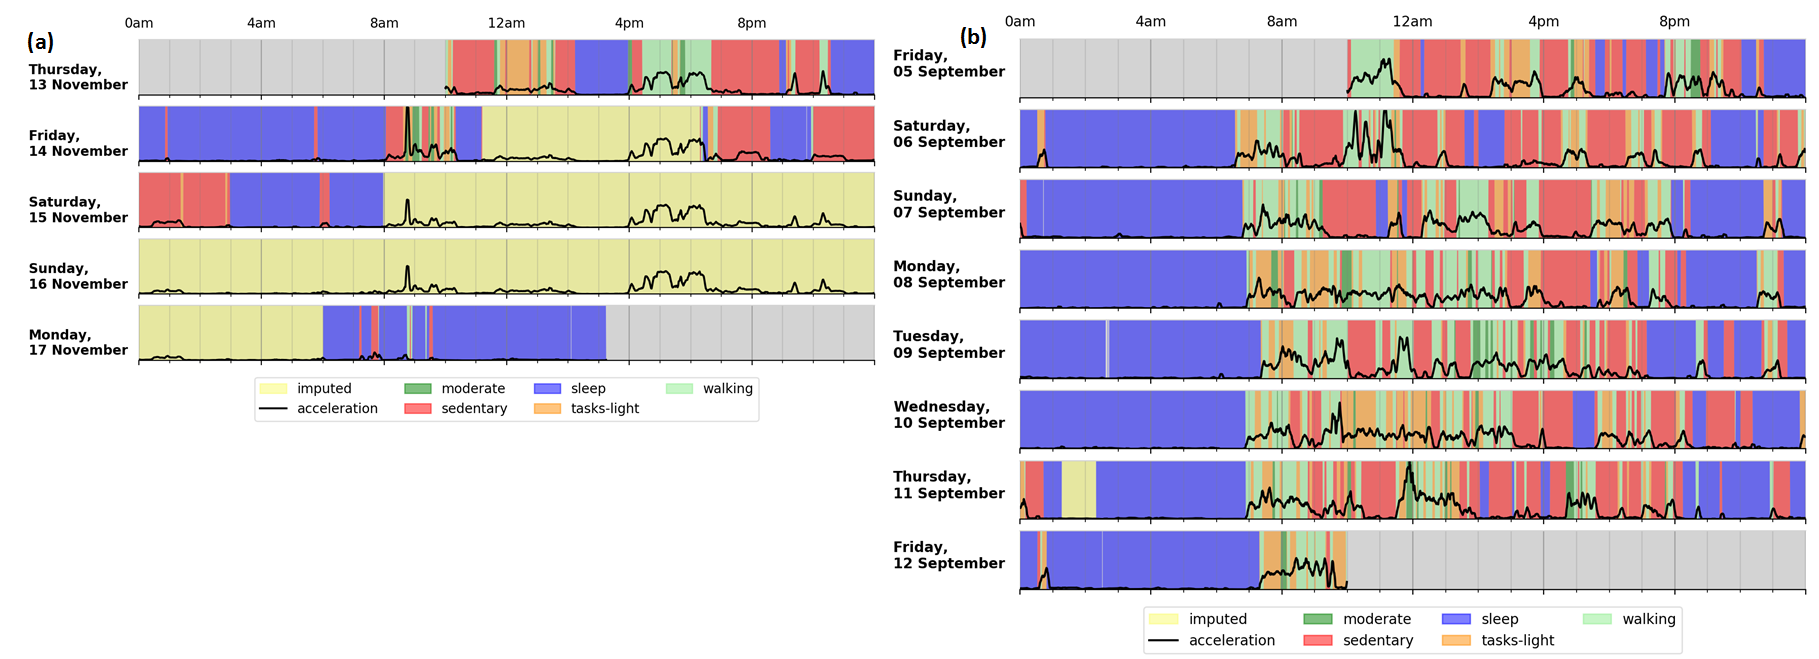
\includegraphics[width=0.95\textwidth]{images/biobank.png}
  \caption{Illustration of daily activity pattern for one participant. Images generated with toolbox provided by \cite{Doherty2017}. The colour code identifies moderate activities, sleep, walking and sedentary patterns. (a) Participant from SMI group. (b) Participant from control group.}
  \label{fig:raw}
\end{figure*}
 
  \subsection{UK Biobank overview}
  The UK Biobank is a very large scale open access database of a wide range genomic and bio-signal records, coming from more than 500,000 people for some data fields. The public showcase of the data available is online at \url{ http://biobank.ctsu.ox.ac.uk/showcase/label.cgi}. In this paper we make use of the physical activity dataset (obtained through UK biobank application number 33693), which was collected from approximately 100,000 people wearing an Activity AX3 3-axis accelerometer device \cite{ref:oAXI19} for a week. During this time participants undertook their normal daily activities and the raw data is unlabelled. All data was sampled at 100~Hz, and both the raw data (in units of g) and a number of derived features (as described below) are available. 

  Also available is a web based questionnaire for these participants, giving information regarding the presence and absence of any mental health condition, including present and past depression, bipolar affective disorder, generalized anxiety disorder, harm behaviour, and subjective wellbeing. The outcomes of these questions are encoded in the Biobank (data field ID 21054) in sixteen fields and allows us to use the raw unlabelled activity dataset in a supervised classification experiment to group participants between SMI and control groups.

  \subsection{Accelerometry features}
  An example of the accelerometery signals available in the dataset, processed using the open source toolbox from \cite{Doherty2017} to threshold the amount of activity into sedentary, moderate, and similar levels of activity, is shown in \fig{feat1}. In addition to the raw data a number of derived features based upon averaging are available including: daily acceleration averages (7~measurements); per hour average acceleration (24 measurements); no-wear time (5 different metrics); categorically encoded age and gender (5 different metrics); overall weekly acceleration average and standard deviation (2 features). The list of all of the features we use, and the associated UK Biobank data fields, is given in \fig{feat1}. As different features have different value ranges we have used a \emph{StandardScaler} normalization applied to the raw data to avoid any potential model bias due to larger values in any individual feature.
  \begin{figure}
    \centering
    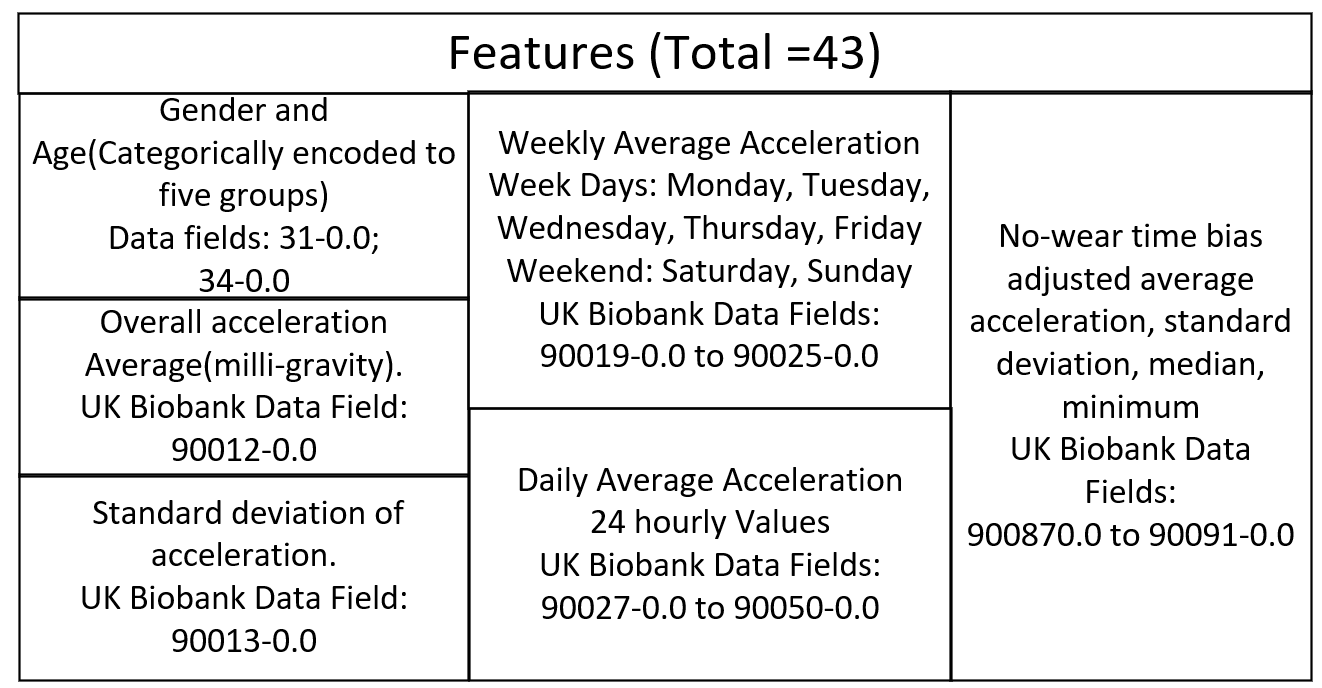
\includegraphics[width=0.47\textwidth]{images/biobank_acc_features-2.png}
    \caption{List of the accelerometer features used in this study and the associated UK Biobank data fields.} 
    \label{feat1}
  \end{figure}

  \subsection{SMI group and control group identification}
  As reported in \cite{Davis2018mhq}, there are 137 participants who indicated any form of mental health condition. Here we make use of the responses to questionnaire A3 and A4 (UK biobank data field 20544-0.1 and 20544-0.2) for which 63 participants (21 female, 42 male) were identified as having an SMI, and use this cohort as our SMI group. 
 
  For the control group, potentially a very large number of participants could be used (all of the remaining participants) but this is computationally impractical for the current work, and it is likely that some participants with undisclosed or undiagnosed SMI would be present in such a control group. Moreover, it would give an extremely imbalanced data set for the machine learning analysis. The machine learning literature proposes to handle data imbalance through either under-sampling or over-sampling strategies. The former involves reducing the majority class by the removal of instances from the training set, while the latter over-samples with repetition from the minority class, thus increasing its impact within the training process. Several variations of under- or over-sampling were proposed in previous studies, including the one-sided Selection and synthetic Minority Oversampling Technique (SMOTE) \cite{witten2016data}.
  
  In this paper we randomly selected a gender matched group of 200 participants from the Biobank to form the control group (86 female, 114 male), giving a dataset of a good size, which is also of a practical size to work with for initial machine learning development.


%%%%%%%%%%%%%%%CNN%%%%%%%%%%%%%%%%%%%%%
\section{Activity based SMI classification} \label{sec:classifier}
In this paper, we utilised an ensemble dense neural network architecture to process the hourly accelerometer features available and classify participants as being in either the SMI or control group. We opted for a DNN architecture due to its capability to process raw time-series data, large error handling capability, and potential for high model accuracy~\cite{RN90}. 

Our model is implemented using the \emph{Keras} open source library in Python \cite{ref:oCHO13}, and we have utilized the \emph{sequential} model and the \emph{dense}, \emph{dropout}, \emph{concetenate}, and \emph{batch normalization} layers. At the very first layer, we fed the 43 features from \fig{feat1}: the thirty-eight derived accelerometer features, one-hot encoded gender (2 channels), and age features (3 channels). These features create a non-linear, distributed representation of the input. A visualisation of the proposed network is given in \fig{fig:model}.
\begin{figure}
  \centering
  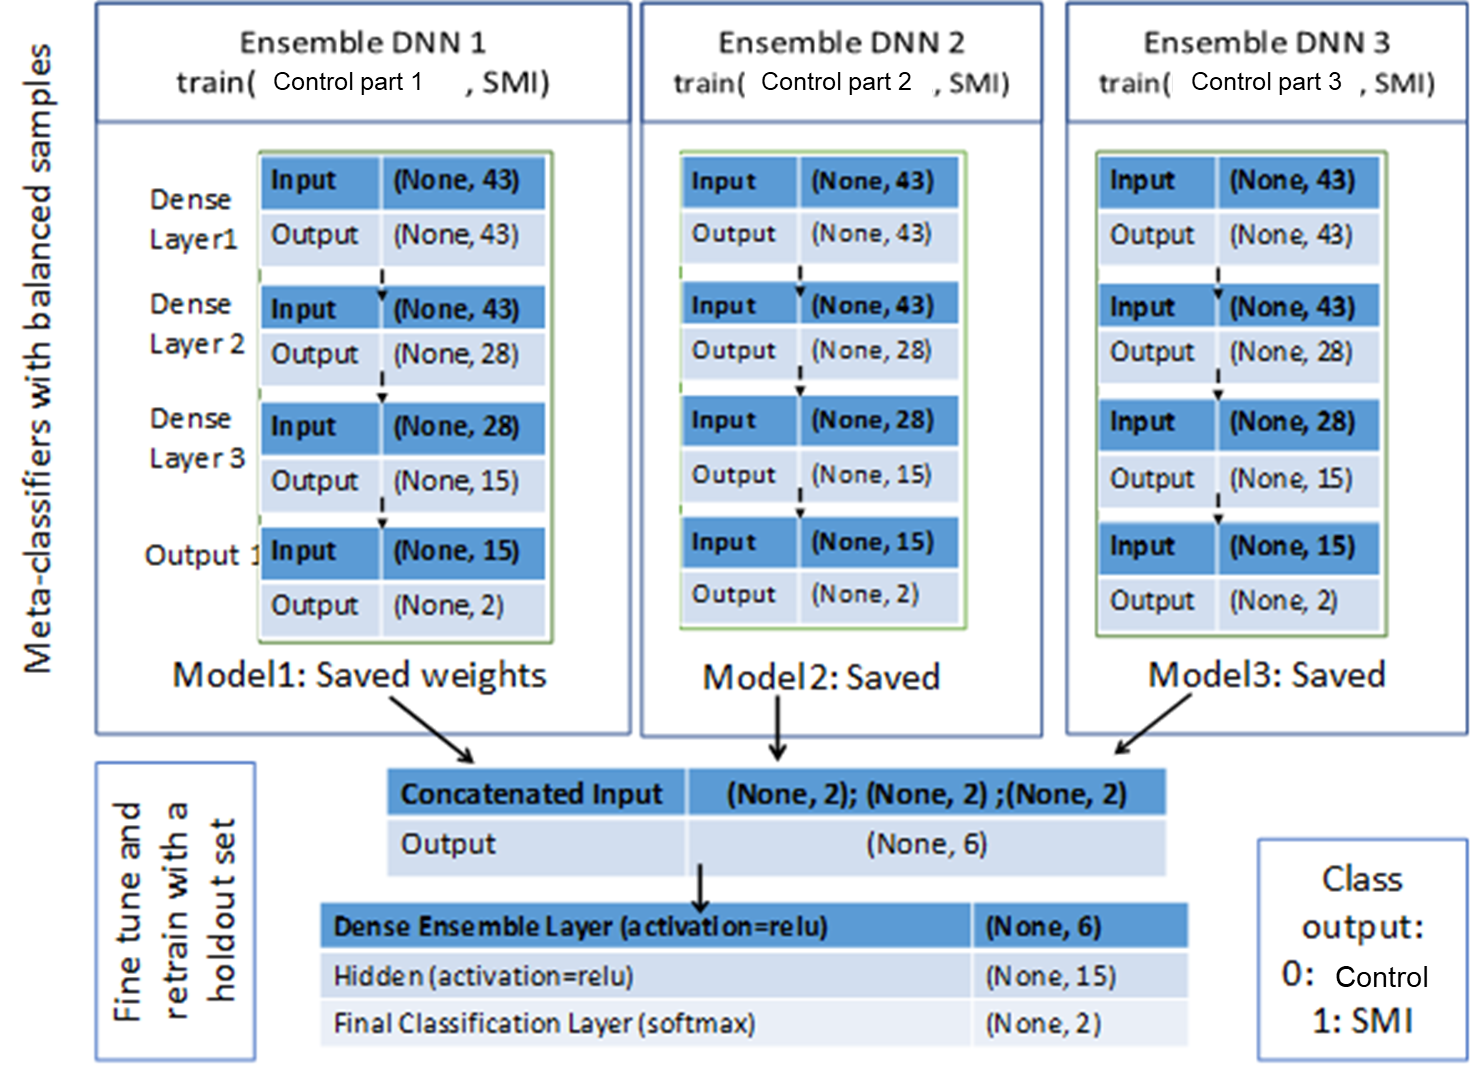
\includegraphics[width=0.47\textwidth]{images/modelArchitecture.png}
  \caption{Visualization of the proposed ensemble Dense Neural Network (DNN) model. The model handles a class imbalance using a synthetic minority oversampling technique.}
      \label{fig:model}
    \end{figure}

Ensemble methods are commonly used for achieving better performance compared to single models. As can be seen from \fig{fig:model}, we started with three baseline models to obtain initial feature processing and classification. In each of these networks there were four dense layers to learn from the features according to their priority. These baseline meta-classifiers were identical in nature for feature exploration purposes, but fed with separate balanced training sets. As the majority (control) group instances (sample size = 200) were almost three times than the minority SMI group (sample size = 63) we partitioned the the majority group into three equal parts to avoid the majority bias on the ensemble layers. We then applied the SMOTE technique on the minority group to further equalize the class imbalance. A balanced test set of 80 participants containing both the groups was kept separately for the purpose of model evaluation.

After the three baseline classifiers a three layer dense neural network is employed (seen at the bottom of \fig{fig:model}), trained by using the concatenated output of the three ensemble DNNs as inputs. This task sequence is retrained in a supervised manner with the class labels and the input feature given to the classifier. We have used a softmax activation layer as the output layer. The layer calculates the loss between the predicted values and the true values, and the weights in the network are adjusted according to the loss. After this stage, all layers are fine-tuned using a holdout dataset through back-propagation in a supervised way. In the test phase, the softmax layer outputs the probability of the predicted categories. The final model was trained with an Adam optimizer with a learning rate of 0.002 and a binary cross-entropy. The training of the model has been done offline on a conventional computer with a 2.4~GHz Intel core i7 processor and 16~GB memory.

To act as comparison cases, in \sect{sec:results} we report the performance of both the ensemble DNN, and a single (non-ensemble) DNN which is identical in set up to the above and trained on the unbalanced training data set. We also report the performance of a standard random forest classifier applied to the data, implemented from the python \emph{sklearn} library. 


%%%%%%%%%%%%%%%%%% RESULTS %%%%%%%%%%%%%%%%%%
\section{Results and discussion} \label{sec:results}
To illustrate the two groupings, we present a comparative pair-plot for weekday and weekend average acceleration for the control and SMI group participants in \fig{feat2}. The control group is seen to have greater average daily acceleration than the SMI group.
 \begin{figure}
    \centering
    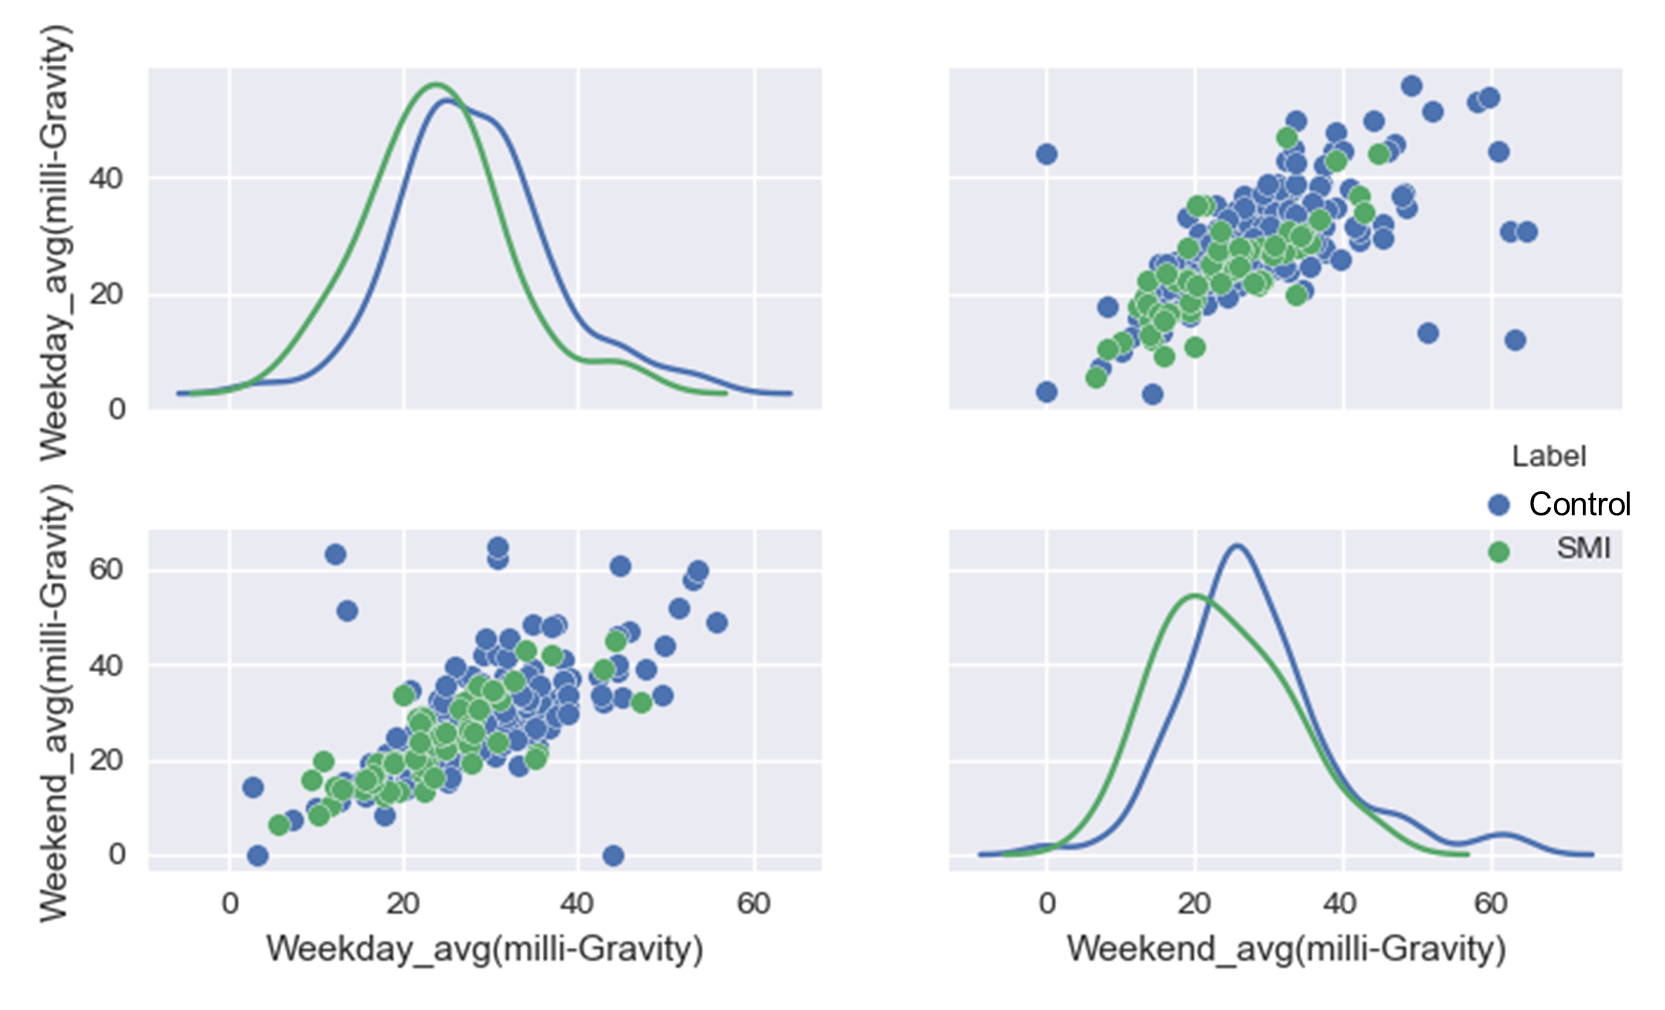
\includegraphics[width=0.49\textwidth]{images/Figure_1.png}
    \caption{Comparative pair-plot for weekday and weekend average acceleration for the control (blue) and SMI (green) participants.} 
    \label{feat2}
  \end{figure} 

Confusion matrices for the single DNN model and ensemble DNN model are given in \fig{fig:confusionmatrix}. It can be seen that the ensemble DNN substantially outperforms the single DNN with an overall accuracy of 91.3\% compared to 83.8\%. The number of records correctly classified into the control state is in fact the same between the two DNN set ups, with the ensemble DNN getting better performance due to more participants being correctly classified into the SMI class.

A comparison to the performance of a random forest classifier is given in \tab{table:performance_comparison}. The random forest model outperformed the single DNN in overall performance, but not the ensemble DNN. In addition, the random forest had much lower recall in the SMI class than either of the DNN based approaches. In terms of model execution time, the ensemble-DNN model took longer (10.9 seconds) in the training phase than the single DNN (3.41 seconds) and random forest (9.66 seconds). 
\begin{table*}
\centering
\caption{Quantitative comparison of ensemble DNN with traditional single DNN and a random forest classifier.}   \label{table:performance_comparison}
 \begin{tabular}{lccccc}
    \toprule
    Classifier &  Overall accuracy & Recall (SMI class) & Recall (Control class) & Precision (SMI class) & Precision (Control class) \\
    \otoprule
          Random forest &  85.2\%  & 67.1\%  & 87.0\%& 64.2\%& 83.0\%\\
     \midrule
    
     Single DNN &   83.8\% & 85.3\% &82.4\%& 84.4\%&78.8\%\\
     Ensemble DNN  &  91.3\% & 89.7\%& 92.7\% & 92.1\%&90.5\%\\
     
    \bottomrule
  \end{tabular}
\end{table*} 

\begin{figure}
  \centering
  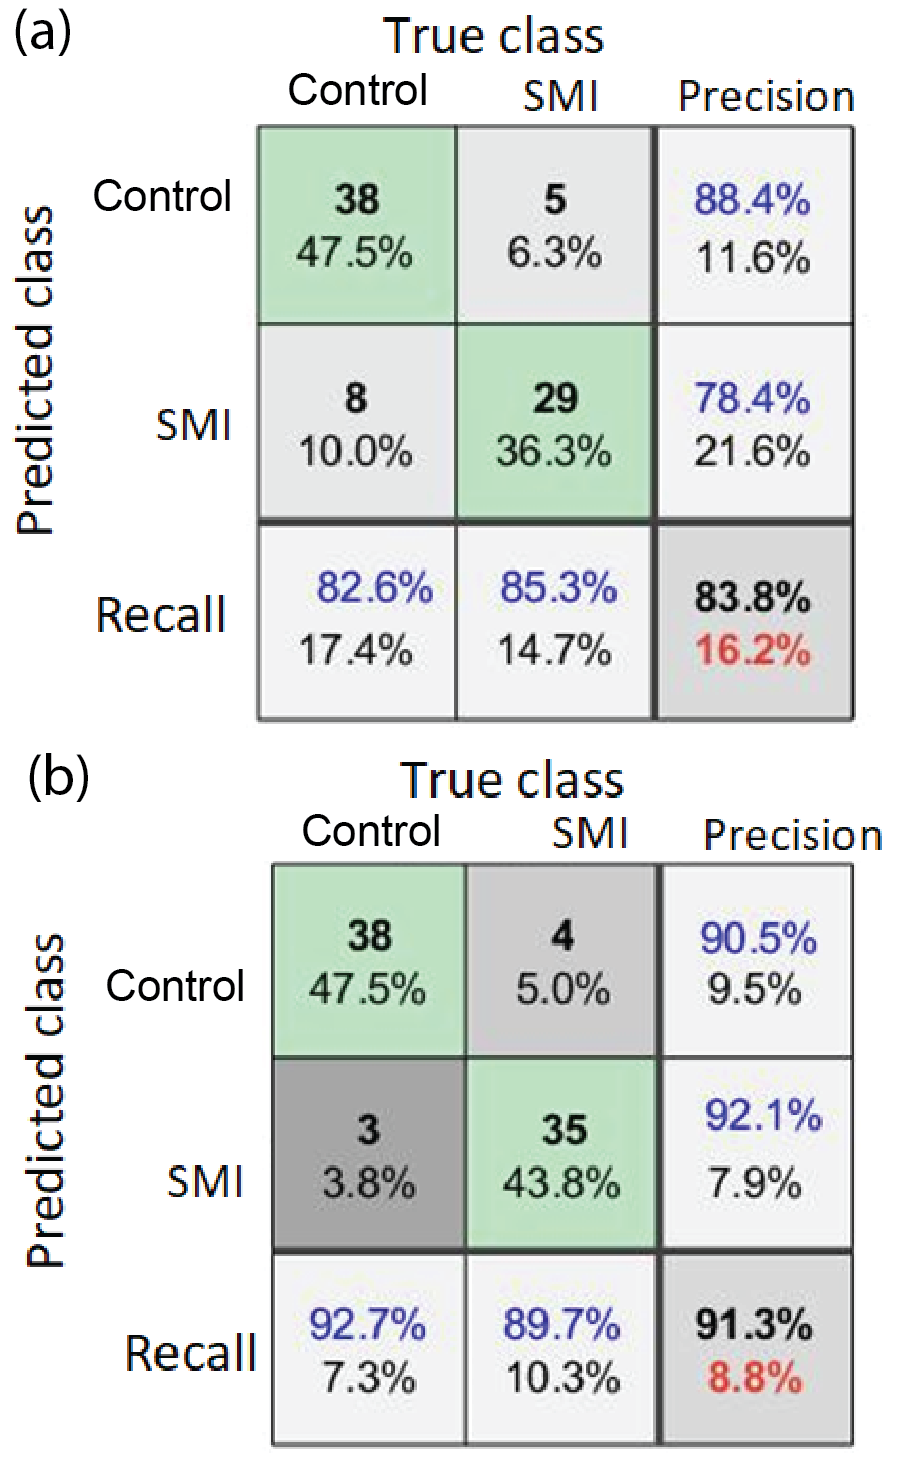
\includegraphics[width=0.25\textwidth]{images/confusion_matrix2.png}
  \caption{Class-wise confusion matrix of the test dataset for the non-ensemble and ensemble DNN.}
  \label{fig:confusionmatrix}
\end{figure}

These high classification performances show that it is possible to differentiate between the two classes based upon a week of activity data. This acts as a starting point to show that there is potential separability between the two classes. Future investigations will look at how this performance changes over time, and whether the accelerometry data sampled at different points in time could be used to give an indicator of potential relapse or remission events, with the ultimate aim of using wearables to help with earlier interventions.



 
%%%%%%%%%%%%%%%%%% CONCLUSIONS %%%%%%%%%%%%%%%%%%
\section{Conclusions} \label{sec:conclusions}
In this work we applied a data-driven ensemble dense neural network technique aimed to identify a serious mental illness participant group from a control group using their physical activity data available from the UK Biobank. This shows that the two classes are potentially separable based upon accelerometer activity recorded over a week. Using an ensemble classifier approach substantially improved the performance compared to using a single dense neural network. This may help with the use of wearable data to compliment smartphone and other mHealth tools currently used in the management of these chronic conditions. 




%%%%%%%%%%%%%%%%%% REFERENCES %%%%%%%%%%%%%%%%%%
\renewcommand*{\bibfont}{\small}
\printbibliography

\end{document}
